\documentclass[a4paper]{article}

\usepackage{listings}
\usepackage{graphicx}
\usepackage{float}
\usepackage[hidelinks]{hyperref}

%opening
\title{Deep Reinforcement Learning Tutorial \\Installation Guide}
\author{Julian Bernhardt, Robin Guth}

\begin{document}

\maketitle
\tableofcontents

\section{Introduction}
Deep Reinforcement Learning (also called RL) is a huge step towards the creation of an universal artificial intelligence. In 2013 a company, owned by Google called ''Deep Mind'', was able to create an astonishing implementation of RL, which was capable to play retro games of the console ''Atari 2600''. In many cases the AI \footnote{Artificial Intelligence} was not only able to play the games successfully, but also exceeded human performances significantly \cite{atari}.\\
As a fairly new topic, beginners often struggle to find a good starting point into the world of AI and specifically RL. Many tutorials are written for more advanced users, who already know basics of machine learning. The ''Deep Reinforcement Learning Tutorial" will provide an easy-to-follow, hands-on beginners guide to RL. After the completion, we will be able to write our own algorithm to play some basic games for us.\\
This installation guide will lead the reader through the setup process for the tutorial. It is also possible to use this as a base for different Machine Learning base, as we will install many standard utilities.
\paragraph{Prerequisites}
It is recommended that the reader already acquired some basic knowledge about programming with Python and is familiar with basic deep learning concepts like Un-/Supervised Learning or at least with basic concept of AI. It is also useful to be able to perform some basic Linux commands, as we will use them later to install some additional packages.
\paragraph{Outlook}
The user will get to know basic concepts of RL with the help of the following programs/utilities/libraries:
\begin{description}
	\item[Python3] One of the most popular programming languages for deep learning. The following tutorials will be based on Python. See \url{https://www.python.org/} for more information.
	\item[Pip] A package installer for Python, which will download and install packages for us from a repository.
	\item[Jupyter Lab] Enables execution of Python code inside a document, used to teach theory and implementation. 
	\item[Google Cloud] Cloud based processing power for training of different implementations of RL. Delivers a linux environment with preinstalled utilities for deep learning including different libraries for Python, Python itself and Jupyter Lab.
	\item[Keras] Framework, which delivers different premade algorithms.
	\item[OpenAiGym] A framework to train and evaluate different AI-based algorithms
\end{description}  
\section{Installation}
\subsection{Google Cloud}
As "Reinforcement Learning" is pretty resource-intensive, Google Cloud will deliver the required performance in the cloud. Python itself, all libraries required and Jupyter Lab need to be available. Luckily, Google already provides a template for a Linux Virtual Machine, which we can use as base for this tutorial. You will have to create a Google account to use the cloud.\\
It is also possible to use this tutorial locally. You will have to prepare a Jupyter Lab environment with the help of PIP or Anaconda and install all required libraries manually. Both are package installers for Python. Check this tutorial \url{https://jupyterlab.readthedocs.io/en/stable/getting_started/installation.html} for more information.
\subsubsection{Deep Learning VM}
To get started in the most simple way, we will use the Google "Deep Learning VM" template to create our environment. It can be found at \url{https://cloud.google.com/deep-learning-vm} or alternatively you can search for "Deep Learning VM" in the Google Cloud marketplace, as shown in picture \ref{fig_marketplaceSearch}.
\begin{figure}[H]
	\centerline{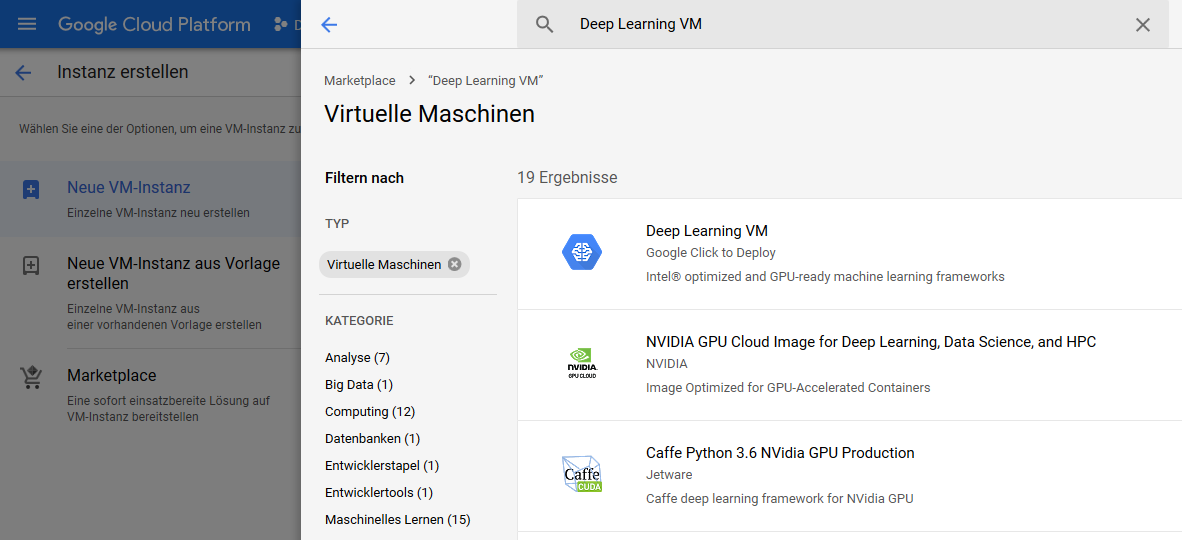
\includegraphics[width=\textwidth]{img/marketplaceSearch}}
	\caption{Searching for ''Deep Learning VM''}
	\label{fig_marketplaceSearch}
\end{figure}
\noindent After you choose the virtual machine, you will be provided with some additional information. Choose ''start in compute engine'' as shown in picture \ref{fig_additionalInfo}.
\begin{figure}[H]
	\centerline{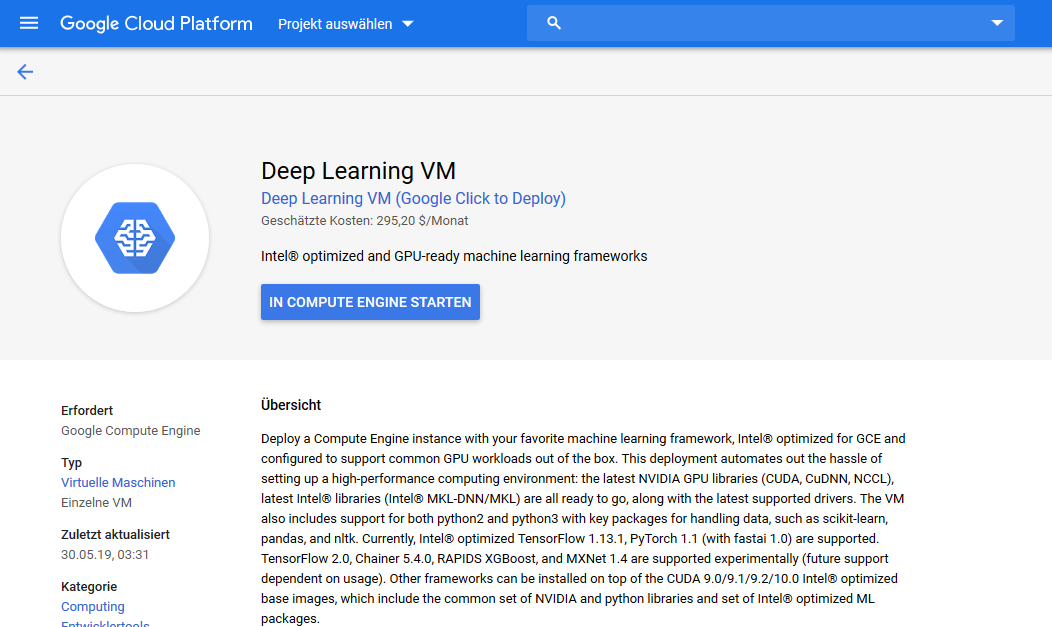
\includegraphics[width=\textwidth]{img/additionalInfo}}
	\caption{After Selecting ''Deep Learning VM''}
	\label{fig_additionalInfo}
\end{figure}
You will be presented with the final configuration screen as shown in picture \ref*{fig_finalConfig} . We need to configure the following options:
\begin{itemize}
	\item Choose a name for your virtual machine
	\item Choose any number of CPU/GPU you want to use (1 CPU is enough)
	\item Choose TensorFlow 1.13 as framework
	\item Activate: ''Install NVIDIA GPU Driver automatically on first startup?''
	\item Activate: ''Enable access to JupyterLab via URL instead of SSH.''
	\item Choose a proper size for the boot disk (minimum of 30 GB is enough)
\end{itemize}
\begin{figure}
	\centerline{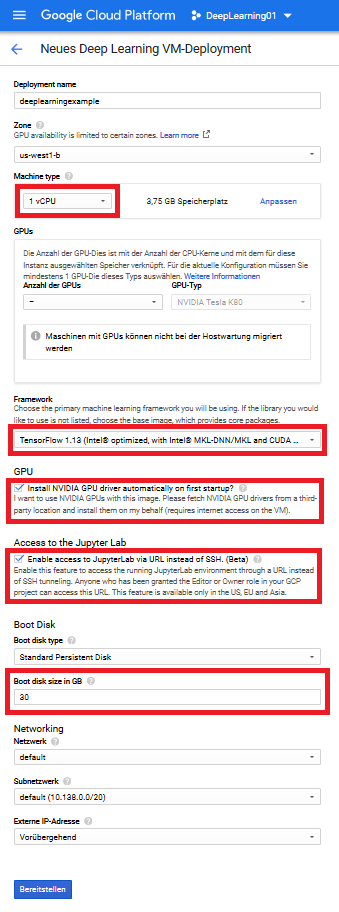
\includegraphics[scale=0.92]{img/finalConfig}}
	\caption{Final Configuration Screen}
	\label{fig_finalConfig}
\end{figure}
\paragraph{Starting the VM}
The VM will start automatically after creating it. It can also be started  manually by selecting it in the vm instances menu and pressing the start button, as shown in picture \ref{fig_startVM}.
\begin{figure}[H]
	\centerline{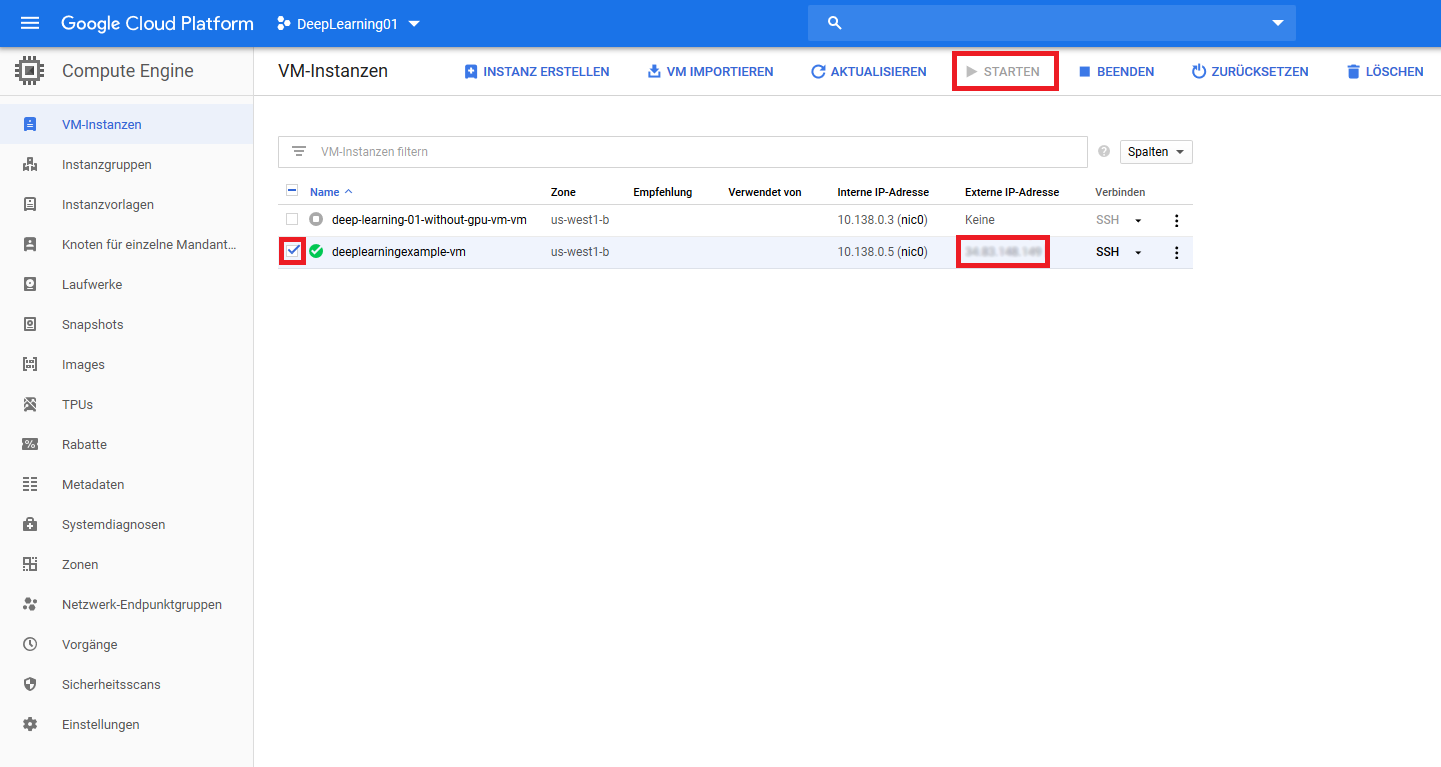
\includegraphics[width=\textwidth]{img/startVM}}
	\caption{Starting the VM}
	\label{fig_startVM}
\end{figure}
\subsubsection{Installing Additional Software}
After we successfully created our first virtual machine instance, we need to install some additional software on the virtual machine. This is possible through an administrator console, which can be opened by clicking the ''SSH'' button in the ''virtual machine instances'' sub-menu, as shown in picture \ref{fig_adminConsole}. The open console can be seen in picture \ref{fig_adminConsole2}.\\
\begin{figure}[H]
	\centerline{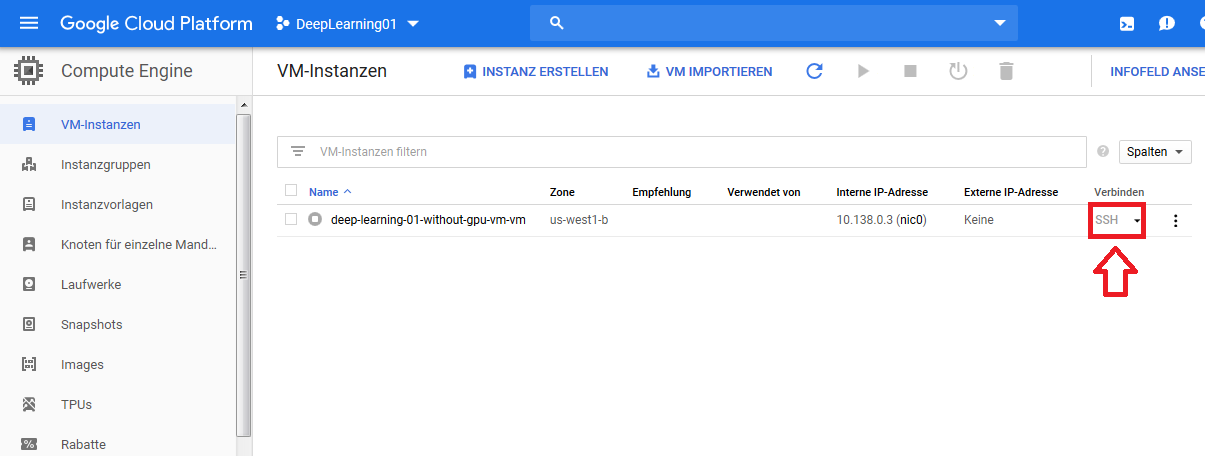
\includegraphics[width=\textwidth]{img/adminConsole}}
	\caption{The ''SSH'' button}
	\label{fig_adminConsole}
\end{figure}
\begin{figure}[H]
	\centerline{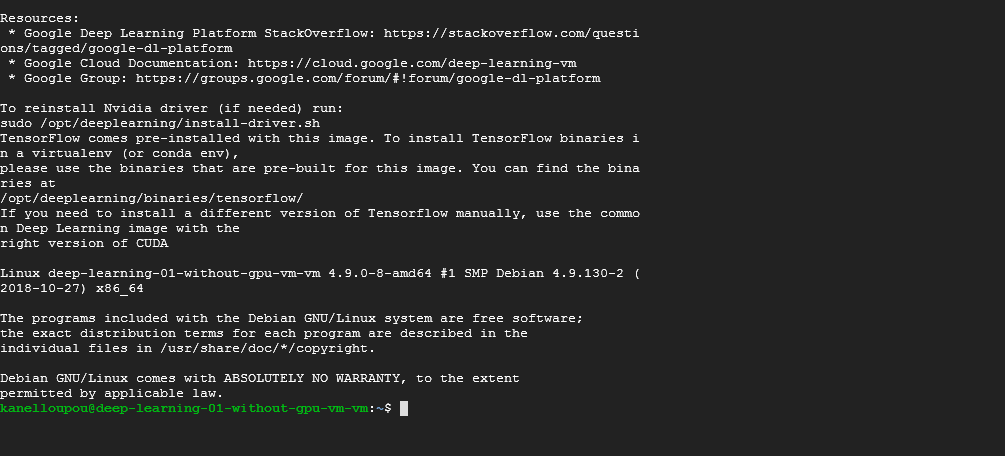
\includegraphics[width=\textwidth]{img/adminConsole2}}
	\caption{The administrator console}
	\label{fig_adminConsole2}
\end{figure}
We need to execute the following commands:
\begin{itemize}
	\item \lstinline|sudo apt-get install python-opengl|
	\item \lstinline|sudo apt-get install xvfb|
\end{itemize}
This will install both python-opengl and xvfb with root rights on our server. We may need to allow the installation by entering ''y'', if the console requests it.  As the Google Cloud server does not provide a display or Open-Gl graphics drivers, we need these programs to run OpenAiGym with visible training/evaluation.\\
After the installation we can finally use Jupyter Lab.
\subsection{Jupyter Lab}
We can connect to Jupyter Lab through the external address that is displayed in the vm instances menu and the port 8080 as shown in picture \ref{fig_startVM}. The address can be entered into a web browser as follows: \lstinline|<external-address>:8080|.
\subsubsection{Upload Notebooks}
After connecting to Jupyter Lab you will be presented with the main menu of Jupyter Lab as shown in picture \ref{fig_mainMenu}. We can now upload the supplied "Deep Reinforcement Learning" notebooks either by using the upload button in the left upper corner or drag and drop to files into the filebrowser. The notebooks can now be opened and used.
\begin{figure}[H]
	\centerline{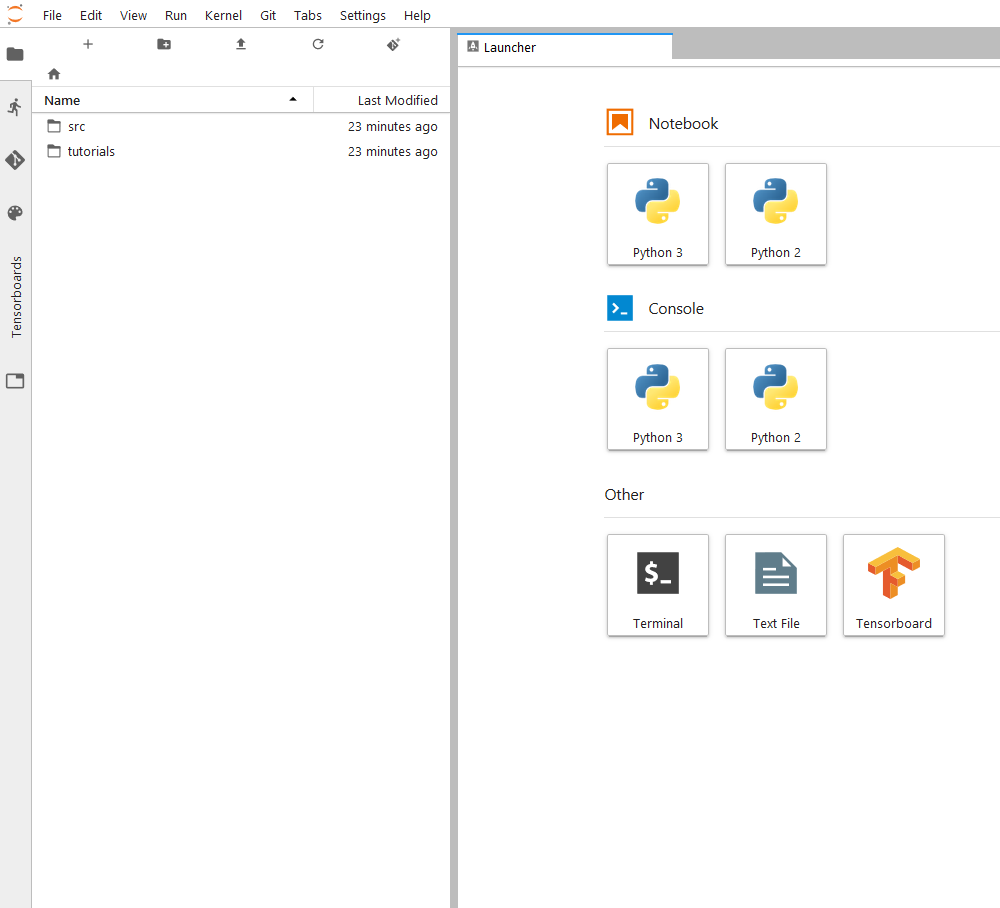
\includegraphics[width=\textwidth]{img/jupyterLab}}
	\caption{Main Menu}
	\label{fig_mainMenu}
\end{figure}
\section{Conclusion}
We have now successfully set up the Google Cloud VM and fetched all dependencies that need to be installed manually. All other libraries will be automatically downloaded while using the notebooks. We can now continue with the first notebook.

\bibliography{bib} 
\bibliographystyle{ieeetr}
\end{document}
